\chapter{Camera Color Calibration}
\label{ch:calibration}

From the previous chapters, we have learned that creating a digital image requires a lot of effort both in the digital and physical worlds. Although automation has proven to be helpful in precise manufacturing and quality evaluation, errors are still bound to happen in the process. Since the camera processes the incoming light sequentially, from optical elements to the ISP, the errors accumulate and amplify at each process step. For this purpose, it is often helpful to calibrate each camera with regard to some reference, such as a device representing the mean of a manufacturing lot or the human visual system.

Camera calibration is a broad field due to different applications having different needs. For example, it might be advantageous to sacrifice colour saturation for noise in autonomous applications, where details are more important. Another application might be to find a camera's intrinsic or extrinsic parameters, which help us relate the corresponding pixels of cameras to produce a depth image. Here, we focus purely on colour-related errors, such as noise and aberrations.

\section{Sources of error}

A typical camera calibration problem is to measure or estimate the spectral responsivities (often known as camera characterization) of an image sensor of interest, such as the ones seen in figure \ref{fig:qe}. After acquiring the responsivities, one could then perform corrections to match the ones of the HVS from figure \ref{fig:xyz}, and apply this same correction to the remaining cameras. This approach, however, is naïve as it does not consider that there might be variability between different realizations of the same product. It is thus crucial to perform some calibration for each camera unit produced under conditions that are reproducible to mitigate the errors caused by the environment.

\subsection{Noise}

Noise is perhaps the most commonly known source of error in all electrical devices. We often use the Signal-to-Noise ratio (SNR) as a metric to quantify the amount of noise in an image, which is often given in decibels (dB) as follows:

\begin{equation}
\label{eq:snr}
SNR = 20\cdot \log_{10}(\frac{\mu}{\sigma}),
\end{equation} 

where, for some image location, $\mu$ is the average signal level and $\sigma$ is the standard deviation, for an image taken under some exposure. Various types of noise exist, but here we will briefly mention the most common ones: photon shot noise, dark current noise and read noise \cite[62, chapter. 3]{rowlands2020physics}

In digital image sensors, some of the noise is unavoidable due to the discrete and independent nature of the arrival of photons. This type of noise is called shot noise and follows a Poisson distribution:

\begin{equation}
\label{eq:poisson}
P(k; \lambda) = \frac{\lambda^k e^{-\lambda}}{k},
\end{equation}

where $\lambda$ is the mean number of photons incident on the sensor for a given period and $k$ is the number of photons that were incident during the current period. The function then gives us the probability of having $k$ photons incident on the sensor. For this distribution, the variance is equal to the average, and so the standard deviation is the square of the mean, $\sigma = \sqrt{\lambda}$. Consequently, the SNR decreases as the average count of photons increases, since the noise only grows as a square of the average signal level. This is why noise is most prevalent when imaging in low-light conditions. \cite[62, chapter. 3]{rowlands2020physics}

Another noise source, mostly prevalent at long exposures, is dark noise. This can be observed by covering the camera lens entirely with a lens cap so that no light is incident on the sensor so that one would expect it not to record any voltage. However, this is wrong as the temperature around the sensor may cause electrons to be emitted, so a signal is recorded within the sensor. This type of noise can be characterized by measuring the average signal recorded under environment where no light is incident on the sensor, and then subtracted from the image at capture time. \cite[289]{nakamura}, \cite[63, chapter. 3]{rowlands2020physics}

Read noise, on the other hand, is always present and occurs due to noise from readout circuits of the imaging sensor, such as the amplifiers. This type of noise is also known as noise floor, since it defines the minimum signal level that can be considered as the actual signal, since read noise is additive. For example, if the image sensor records a value of 128 but the noise floor is 8, we would subtract $8$ from $128$, resulting in an output value of $120$. As read noise tends to fluctuate, it can not be measured precisely and thus can not be removed completely from the signal. \cite[pp. 62-63, chapter. 3]{rowlands2020physics}

\subsection{Optical Design}

Errors due to optical systems, such as colorful contours or gradual changes in brightness and color shifts, are often attributed to how light bends when it passes from one medium to another. This phenomenon is governed by Snell's Law, which is typically presented as:

\begin{equation}
\label{eq:snell_revised}
n_1 \sin(\theta_1) = n_2 \sin(\theta_2),
\end{equation}

where $n_1$ and $n_2$ are the refractive indices of the first and second media, respectively, and $\theta_1$ and $\theta_2$ are the angles of incidence and refraction relative to the normal to the interface between the two media. However, dispersion is often omitted when discussing Snell's law, which specifies the refractive index $n$ to depend on the light's wavelength $\lambda$. The refractive index can be more accurately represented as $n(\lambda)$, indicating its dependence on the wavelength. Therefore, a more precise formulation of Snell's Law that accounts for dispersion would include the wavelength dependence of the refractive indices:

\begin{equation}
\label{eq:snell_wavelength}
n_1(\lambda) \sin(\theta_1) = n_2(\lambda) \sin(\theta_2).
\end{equation}

This wavelength-dependent refractive index explains why light's different colours (wavelengths) bend at slightly different angles when passing through optical elements, leading to the optical errors observed in images. Three such errors are visualized in figure \ref{fig:aberration}, where light rays from a ring are first incident on a convex lens, and finally reflected onto the image plane. In the topmost example, the ring is reproduced as it was seen in nature with no optical aberrations, as all light rays converge to the exact same location. In the second case, we see a noticeable blur along the edges of the ring; here different light rays bend at slightly different angles due to dispersion and as a result, each light ray has a different focal length, a phenomenon known as longitudinal chromatic aberration. In the third case, the light rays again converge at different locations due to dispersion, but at the same focal plane, thus this is called lateral chromatic aberration.

\begin{equation}
\label{eq:snell}
n_1  = \frac{c}{v},
\end{equation}

where $c=\approx \SI{3e+8}{\meter\per\second}$ and $v$ is the speed of light in the observed medium.


\begin{figure}
    \centering
    \pdftooltip{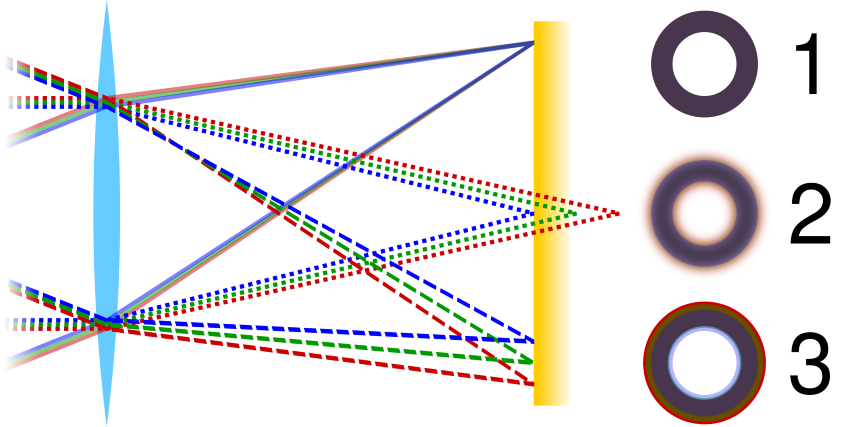
\includegraphics[width=\textwidth]{figures/aberration.png}}{nikon}
    \caption{Optical aberrations}
    \label{fig:aberration}
\end{figure}
